% status: 100
% chapter: Streaming

\title{Real Time Stream Processing - Big Data}

\author{Ravinder Lambadi}
\affiliation{%
  \department{School of Informatics, Computing, and Engineering}
  \institution{Indiana University}
  \city{Bloomington}
  \state{IN}
  \postcode{47408}
  \country{USA}}
\email{rlambadi@iu.edu}


\author{Orly Esteban}
\affiliation{%
  \department{School of Informatics, Computing, and Engineering}
  \institution{Indiana University}
  \city{Bloomington}
  \state{IN}
  \postcode{47408}
  \country{USA}}
\email{oesteban@iu.edu}


\begin{abstract}
Every business organization around the globe are rapidly progressing 
towards taking advantages of big data offerings. 
Big Data characteristics includes high Volume, Variety as well as Velocity of data.  
Big Data needs to be processed fast 
so as to enable organizations to act in real-time for fast paced changing business conditions. 
Big data technologies stack includes 
Open Source Hadoop platform that offers capabilities for storage, distributed data processing, 
data streaming in real-time and computational 
platform for business analytics.  In this paper, an attempt is made to capture real t
ime data streaming process including the components involved in the process along with Industry stream 
processing frameworks and commonly used Streaming products. 
This paper also provides brief on practical use cases for real time stream processing.

\end{abstract}

\keywords{hid-sp18-514,hid-sp18-506, Apache NIFI, Apache Kafka, Apache storm, Apache spark, and Stream processing}

\maketitle

\section{Introduction}

Streaming data is the data that is produced continuously by many data sources 
and includes a wide variety of data such as browser cookie data,
server log files, credit card transactions, data generated from social networks, 
financial trading, data generated by customers using mobile and IOT sensor data.  
When data is continuously bucketing in your organization, we need a huge data warehouse system or HDFS, 
or Apache HBase or any other NON-Relation database server to store it. 
There are two ways to analyze, and process either in batch mode or in 
real time mode depending on organization requirements. 
But most of the organizations are looking for real time actionable analytics to make faster decision
 
\section{Stream Overview}
''The data needs to be processed sequentially and incrementally on a record-by-record basis or over sliding time windows, 
and used for a wide variety of analytics including correlations, aggregations, filtering, and sampling. 
Information derived from such analysis gives companies visibility into many aspects of their business and customer activity 
such as -service usage (for metering/billing), server activity, website clicks, and geo-location of devices, people, and physical g
oods -and enables them to respond promptly to emerging situations. For example, businesses can track changes in public sentiment 
on their brands and products by continuously analyzing social media streams, 
and respond in a timely fashion as the necessity arises''~\cite{hid-sp18-514-bigdata-stream-overview}.
 
Below are few of the frameworks and products developed in order to implement data streaming
 
\section{Apache NIFI}
 
NIFI works with Apache Kafka, Apache Storm, Apache HBase and Spark for real-time distributed messaging of streaming data. 
NiFi platform is used for ingesting real-time streaming data sources, such as the internet of things, 
sensors and transactional systems. Nifi has in built tools to filter any un-wanted data during data pre-processing stage

There are four main components of NiFi to consume data for processing and producing the output
 
\begin{itemize}
\item FlowFile
\item Processor
\item Connections
\item And Flow Controller
\end{itemize}
 
\section{NiFi Architecture}

\centering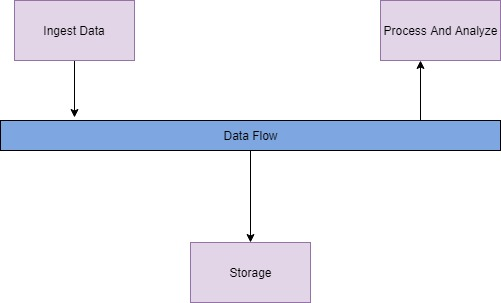
\includegraphics[width=\columnwidth]{images/NiFi.jpg}
 
FlowFile responsible to bring the data in to NiFi from any data sources. 
Connections are link between NiFi components to move within the flow. 
Controller normalizes of FlowFiles between the processes.  Processors are 
action component to process FlowFiles contents and produces output. 
In the enterprise NiFi acts as a producer to publish messages to the topic. 
The messages are broadcasted over the network to the Apache Kafka Cluster.
 
 
\section{Apache Kafka}
''Kafka works in combination with Apache Storm, Apache HBase and Apache 
Spark for real-time distributed messaging of streaming data. 
Kafka is a low latency messaging platform for real-time streaming data sources, 
such as the internet of things, sensors, 
and transactional systems. Kafka brokers huge message streams for low-latency 
analysis in Enterprise Apache Hadoop ecosystem''~\cite{hid-sp18-514-hwp}.
 
\section{Apache Storm}
Apache storm is a real time distributed computational system for processing huge volume of data in parallel 
and with high scalability. Initially it was developed by twitter and it is composed of other open source components.
Storm provides an interface for developers to develop applications that analyze streams of data (multiple rows). 
A row may contain any objects type.
''At the core of Storm's data stream processing is a computational topology, which is discussed below. 
This topology of nodes dictates how tuples are processed, transformed, aggregated, stored, or re-emitted to 
other nodes in the topology for further processing''~\cite{hid-sp18-514-hwp}

Below characteristics of Storm ideal for real-time data processing workloads:

\begin{itemize}
\item Fast
\item Scalable
\item Fault-tolerant
\item Reliable
\end{itemize}
 
Storm has three sets of components, each them have own responsibility during processing. Nimbus node uploads 
computation for execution, code distribution, launch workers, monitor and reallocates 
workers based on load in the cluster.
ZooKeer co-ordinates the storm cluster in the enterprise. Supervisor node, 
interact with Nimbus through ZooKeeper to manage workers according direction from Nimbus.

\centering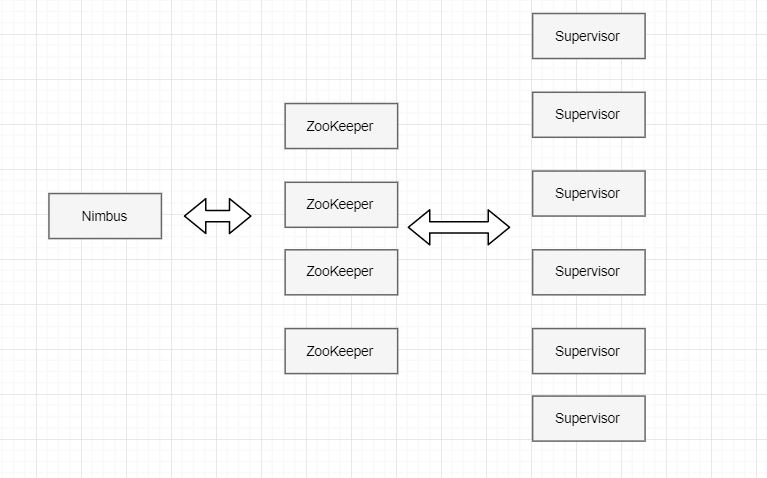
\includegraphics[width=\columnwidth]{images/Storm1.JPG}

  
Five key abstractions help to understand how Storm processes data

\begin{itemize}
\item Tuples : An ordered list of elements.
\item Streams : ''An unbounded sequence of tuples''~\cite{hid-sp18-514-hwp}
\item Spouts : ''Sources of streams in a computation (e.g. a Twitter API)''~\cite{hid-sp18-514-hwp}
\item Bolts : ''Process input streams and produce output streams. They can run functions, filter, aggregate, or join data, or talk to databases''~\cite{hid-sp18-514-hwp}
\item Topologies: ''The overall calculation, represented visually as a network of spouts and bolts''~\cite{hid-sp18-514-hwp}
\end{itemize}

\section{Apache Spark}
Apache spark is a framework for large-scale data processing that supports several different
programming languages and concepts such as Hadoop Map Reduce, distributed in-memory processing, 
stream processing, and machine learning. This can be used on top the Hadoop framework

\section{Other Stream Processing Frameworks and Products}

\begin{itemize}
\item Apache Samza
\item Esper 
\item AWS Kinesis 
\item Data Torrent 
\item And Oracle CEP 
\end{itemize}


\section{User Case}
Real time audience selection based on browse pattern in the web (credit card recommendation)

\section{High Level Architecture}
Data ingestion happens from various sources in real time. Real time audience selection application hosted on Big Data platform.
Bluekai (Oracle) posts cookie data to this application through REST API continuously. This application performs pre-processing, 
validation, and then perform actual processing in real time and then find the selected 
audience based on cookie data and business rules and post back recommended audience to Bluekai

\centering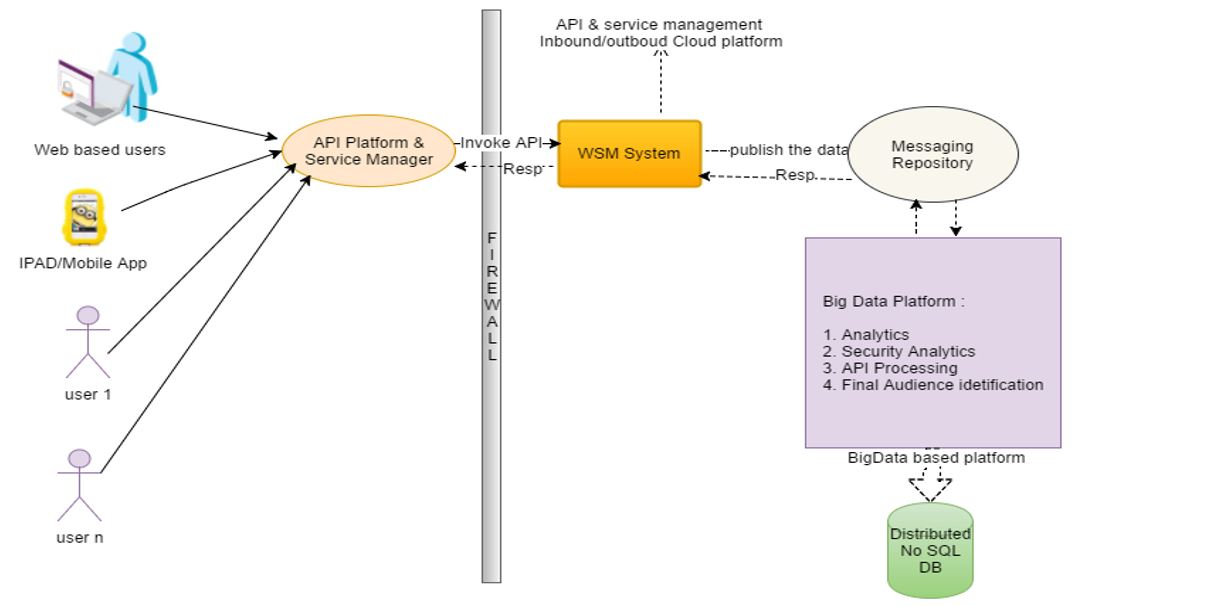
\includegraphics[width=\columnwidth]{images/realTimeAudienceSelection.JPG}

 
\section{Conclusion}
Stream processing is required when data has to be processed continuously in a real time. There are several open source, 
commercial frameworks and products available in the industry for real time stream processing. In this paper, an attempt is made 
to describe Hortonworks streaming components, NiFi ingests, route and land real time data streaming. Kafka captures and perform instant 
processing with Apache Storm. This paper also provided one use case for real time audience selection using Big Data platform

\begin{acks}

  The author would like to thank Dr.~Gregor~von~Laszewski for his
  support and suggestions to write this paper.

\end{acks}

\bibliographystyle{ACM-Reference-Format}
\bibliography{report} 
